\documentclass{beamer}

\usepackage[T1]{fontenc} 
\usepackage[latin1]{inputenc}
%% \usepackage[frenchb]{babel}

\usetheme{Warsaw}

% Supprimer les icones de navigation (pour les transparents)
\setbeamertemplate{navigation symbols}{}

\usepackage{tikz}
\usetikzlibrary{decorations, decorations.pathreplacing, decorations.pathmorphing, shapes}

\title[Introduction {\`a} la Bio-Informatique]{Introduction {\`a} la Bio-Informatique}
\author{Gabriel Chandesris}
%% \institute{ --- }
\institute{ 
\includegraphics[height=0.5cm]{img/logo_glider.png} }
%% \logo{ 
\includegraphics[height=2.5cm]{img/logo_glider.png} }

\date{\today}

\begin{document}

\begin{frame}
	\titlepage
\end{frame}

\begin{frame}
	\frametitle{Contenu de cette pr{\'e}sentation}
	\small \tableofcontents[hideallsubsections]
\end{frame}

\begin{frame}
	\frametitle{ Vision G{\'e}n{\'e}rale du cours et Sources d'inspiration }
	
	\begin{columns}[T]
	\begin{column}[T]{5.0cm}
	
		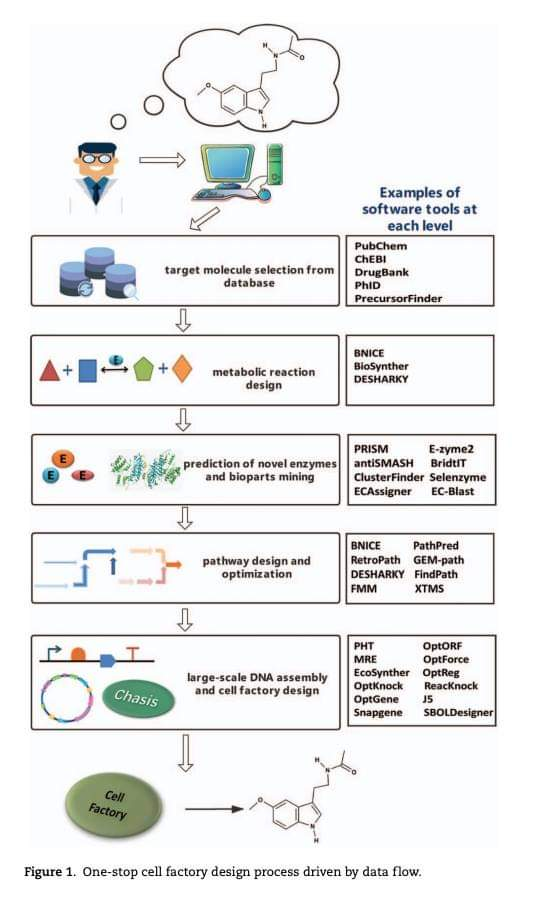
\includegraphics[width=4.0cm]{resources/BioInformaticsWorkflowWithTools.jpg} 
	
	\end{column}
	\begin{column}[T]{7.5cm}
	
		\begin{itemize}
			\item Plan du programme du contenu du module 6 du BTS Biotechnologies (et ressources associ{\'e}es) ;  
			\item Cours de licence Bio-Informatique du CNAM (Conservatoire National des Arts et M{\'e}tiers) ; 
			\item ... 
		\end{itemize}
		
		\end{column}
	\end{columns}
\end{frame} 
%%%%% %%%%% %%%%% %%%%% %%%%% PARTIE 0 %%%%% %%%%% %%%%% %%%%% %%%%% 

\def\titleSection0{Rappels de Biologie / Biochimie et Parcours Rapide}
\section{ \titleSection0 }
\begin{frame}
	\frametitle{ \titleSection0 }
	\tableofcontents[sections=1,currentsection,subsectionstyle=show/shaded/hide]
\end{frame} 

\def\titleSection0SubsectionI{Rappels de base de biologie {\`a} usage pour la bio-informatique}
\subsection{ \titleSection0SubsectionI }
\begin{frame}
	\frametitle{ \titleSection0SubsectionI }
	\begin{itemize}
		\item Les cha{\^i}nes du vivant, ADN et Prot{\'e}ines.
		\item La cellule : unit{\'e} fonctionnelle du vivant.
		\item {\'E}l{\'e}ments de physiopathologie : inflammation, maladies infectieuses et cancers
	\end{itemize}
\end{frame}

\def\titleSection0Subsection2{Les grandes banques (bases de donn{\'e}es) bio-informatiques}
\subsection{ \titleSection0Subsection2 }
\begin{frame}
	\frametitle{ \titleSection0Subsection2 }
	\begin{itemize}
		\item Banques de donn{\'e}es disponibles sur Internet : s{\'e}quences, polymorphismes, structure des prot{\'e}ines. 
		\item Le syst{\`e}me Entrez : du g{\`e}ne {\`a} la fonction. \texttt{https://www.ncbi.nlm.nih.gov/Web/Search/entrezfs.html}
		\item ... 
	\end{itemize}
\end{frame}

\def\titleSection0Subsection3{Exploitation des banques de s{\'e}quences et applications}
\subsection{ \titleSection0Subsection3 }
\begin{frame}
	\frametitle{ \titleSection0Subsection3 }
	\begin{itemize}
		\item Les logiciels disponibles sur Internet : criblage de banque, alignement de deux s{\'e}quences, phylog{\'e}nie. Principes algorithmiques et utilisation.
		\item ... 
	\end{itemize}
\end{frame}

\def\titleSection0Subsection4{Mod{\'e}lisation mol{\'e}culaire et applications}
\subsection{ \titleSection0Subsection4 }
\begin{frame}
	\frametitle{ \titleSection0Subsection4 }
	\begin{itemize}
		\item Logiciels de r{\'e}f{\'e}rence (RasMol, Cn3D, VMD). Pr{\'e}diction de structure, m{\'e}thodes automatiques.
		\item ... 
	\end{itemize}
\end{frame}

\def\titleSection0Subsection5{Probl{\'e}matiques Bio-informatiques li{\'e}es aux nouvelles technologies}
\subsection{ \titleSection0Subsection5 }
\begin{frame}
	\frametitle{ \titleSection0Subsection5 }
	\begin{itemize}
		\item S{\'e}quen\c{c}age massif du g{\'e}nome  (Next Generation Sequencing, NGS), puces de g{\'e}notypage, puces de transcriptome, g{\'e}nomique sur cohorte et maladies, g{\'e}n{\'e}tique d'association, initiation {\`a} l'utilisation des donn{\'e}es NGS avec Galaxy.
		\item ... 
	\end{itemize}
\end{frame}


%%%%% %%%%% %%%%% %%%%% %%%%% PARTIE 1 %%%%% %%%%% %%%%% %%%%% %%%%% 

\def\titleSection1{Notions de base (informatique)}
\section{ \titleSection1 }
\begin{frame}
	\frametitle{ \titleSection1 }
	\tableofcontents[sections=2,currentsection,subsectionstyle=show/shaded/hide]
\end{frame} 

\def\titleSection1SubsectionI{Le codage de l'information et la num{\'e}risation des donn{\'e}es (nombres, textes, images ...)}
\subsection{ \titleSection1SubsectionI }
\begin{frame}
	\frametitle{ \titleSection1SubsectionI }
	\begin{itemize}
		\item Fichiers textes ("texte brut" et WYSIWIG) et fichiers binaires
		\item Nombres : repr{\'e}sentation et limites
		\item ... 
	\end{itemize}
\end{frame}

\def\titleSection1Subsection2{Architecture mat{\'e}rielle et logicielle d'un ordinateur}
\subsection{ \titleSection1Subsection2 }
\begin{frame}
	\frametitle{ \titleSection1Subsection2 }
	\begin{itemize}
		\item Unit{\'e} centrale : disque dur, carte m{\`e}re, processeur, carte graphique, carte(s) r{\'e}seau(x) ; 
		\item {\'E}cran et autres {\'e}l{\'e}ments d'affichage (et d'impression) : p{\'e}riph{\'e}riques de sortie ; 
		\item Clavier, souris et autres p{\'e}riph{\'e}riques d'entr{\'e}es ; 
		\item Ordinateurs r{\'e}cents ("iMacs", SmartPhones...) : monobloc ; 
		\item ... 
	\end{itemize}
\end{frame}

\def\titleSection1Subsection3{Les r{\'e}seaux et Internet}
\subsection{ \titleSection1Subsection3 }
\begin{frame}
	\frametitle{ \titleSection1Subsection3 }
	\begin{columns}[T]
	\begin{column}[T]{5.0cm}
	
		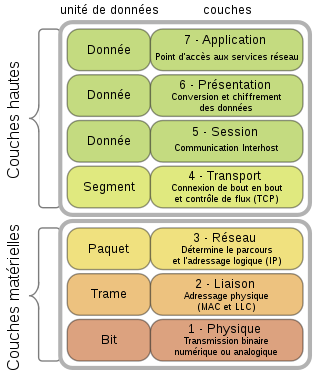
\includegraphics[width=5.0cm]{resources/langfr-330px-OSI_Model_v1.svg.png} 
	
	\end{column}
	\begin{column}[T]{7.5cm}
	
		\begin{itemize}
			\item Couches OSI
			\item Du mat{\'e}riel et du logiciel !
			\item Protocoles d'{\'e}changes (TCP / IP) ; 
			\item Routeurs, R{\'e}seaux Locaux (WAN / LAN) et r{\'e}seau global ; 
			\item ... 
		\end{itemize}
		
	\end{column}
	\end{columns}
\end{frame}

	% \begin{itemize}
	% 	\footnotesize
	% 	\item[Couche 7 -- Applicative] Logiciels. %% C'est {\`a} ce niveau que sont les logiciels: navigateur, logiciel d'email, FTP, chat...
	% 	\item[Couche 6 -- Pr{\'e}sentation] Affichage. %% Elle est en charge de la repr{\'e}sentation des donn{\'e}es (de telle sorte qu'elle soit ind{\'e}pendante du type de microprocesseur ou du syst{\`e}me d'exploitation par exemple) et - {\'e}ventuellement - du chiffrement.
	% 	\item[Couche 5 -- Session] Identificatiion. %% En charge d'{\'e}tablir et maintenir des sessions (c'est {\`a} dire d{\'e}buter le dialogue entre 2 machines: v{\'e}rifier que l'autre machine est pr{\^e}te {\`a} communiquer, s'identifier, etc.)
	% 	\item[Couche 4 -- Transport] Liaison. %% En charge de la liaison d'un bout {\`a} l'autre. S'occupe de la fragmentation des donn{\'e}es en petits paquets et v{\'e}rifie {\'e}ventuellement qu'elles ont {\'e}t{\'e} transmises correctement.
	% 	\item[Couche 3 -- R{\'e}seau] Transport. %% En charge du transport, de l'adressage et du routage des paquets.
	% 	\item[Couche 2 -- Liaison de donn{\'e}es] Encodage. %% En charge d'encoder (ou moduler) les donn{\'e}es pour qu'elles soient transportables par la couche physique, et fournit {\'e}galement la d{\'e}tection d'erreur de transmission et la synchronisation.
	% 	\item[Couche 1 -- Physique] Support. %% C'est le support de transmissions lui-m{\^e}me: un fil de cuivre, une fibre optique, les ondes hertziennes...
	% \end{itemize}

\def\titleSection1Subsection4{Fichiers et bases de donn{\'e}es}
\subsection{ \titleSection1Subsection4 }
\begin{frame}
	\frametitle{ \titleSection1Subsection4 }
	\begin{itemize}
		\item Fichier plat, tabulaires, XML, bases relationnelles (SQL)
		\item ... 
	\end{itemize}
\end{frame}

\def\titleSection1Subsection5{Algorithmique}
\subsection{ \titleSection1Subsection5 }
\begin{frame}
	\frametitle{ \titleSection1Subsection5 }
	\begin{itemize}
		\item Programmation : structures de contr{\^o}les, structures de donn{\'e}es, traitement des donn{\'e}es ; 
		\item ... 
	\end{itemize}
\end{frame}

%%%%% %%%%% %%%%% %%%%% %%%%% Recherche, traitement et pr{\'e}sentation de l'information %%%%% %%%%% %%%%% %%%%% %%%%% 

\def\titleSection2{Recherche, traitement et pr{\'e}sentation de l'information}
\section{ \titleSection2 }
\begin{frame}
	\frametitle{ \titleSection2 }
	\tableofcontents[sections=3,currentsection,subsectionstyle=show/shaded/hide]
\end{frame} 

\def\titleSection2SubsectionI{Interrogation d'une banque de donn{\'e}es bibliographiques}
\subsection{ \titleSection2SubsectionI }
\begin{frame}
	\frametitle{ \titleSection2SubsectionI }
	\begin{itemize}
		\item ... 
	\end{itemize}
\end{frame}

\def\titleSection2Subsection2{Traitement de texte}
\subsection{ \titleSection2Subsection2 }
\begin{frame}
	\frametitle{ \titleSection2Subsection2 }
	\begin{itemize}
		\item ... 
	\end{itemize}
\end{frame}

\def\titleSection2Subsection3{Tableur-Grapheur}
\subsection{ \titleSection2Subsection3 }
\begin{frame}
	\frametitle{ \titleSection2Subsection3 }
	\begin{itemize}
		\item ... 
	\end{itemize}
\end{frame}

\def\titleSection2Subsection4{Utilisation d'un logiciel de pr{\'e}sentation}
\subsection{ \titleSection2Subsection4 }
\begin{frame}
	\frametitle{ \titleSection2Subsection4 }
	\begin{itemize}
		\item ... 
	\end{itemize}
\end{frame}

%%%%% %%%%% %%%%% %%%%% %%%%% Acquisition de donn{\'e}es et gestion de proc{\'e}d{\'e}s %%%%% %%%%% %%%%% %%%%% %%%%% 

\def\titleSection3{Acquisition de donn{\'e}es et gestion de proc{\'e}d{\'e}s}
\section{ \titleSection3 }
\begin{frame}
	\frametitle{ \titleSection3 }
	\tableofcontents[sections=4,currentsection,subsectionstyle=show/shaded/hide]
\end{frame} 

\def\titleSection3SubsectionI{Contr{\^o}le et commandes (automates, bior{\'e}acteurs...)}
\subsection{ \titleSection3SubsectionI }
\begin{frame}
	\frametitle{ \titleSection3SubsectionI }
	\begin{itemize}
		\item ... 
	\end{itemize}
\end{frame}

\def\titleSection3Subsection2ACRO{TAI}
\def\titleSection3Subsection2{Traitements et Analyses d'Images (TAI)}
\subsection{ \titleSection3Subsection2 }
\begin{frame}
	\frametitle{ \titleSection3Subsection2 }
	\begin{itemize}
		\item ... 
	\end{itemize}
\end{frame}


\def\titleSection3Subsection2to1{ TAI : D{\'e}finitions et formats de fichiers}
\subsection{ \titleSection3Subsection2to1 }
\begin{frame}
	\frametitle{ \titleSection3Subsection2to1 }
	\begin{itemize}
		\item ... 
	\end{itemize}
\end{frame}

\def\titleSection3Subsection2subsubsection2{ TAI : Logiciels de traitement (exemple)}
\subsection{ \titleSection3Subsection2subsubsection2 }
\begin{frame}
	\frametitle{ \titleSection3Subsection2subsubsection2 }
	\begin{itemize}
		\item ... 
	\end{itemize}
\end{frame}

\def\titleSection3Subsection2subsubsection3{ TAI : Analyse densitom{\'e}trique d'une image}
\subsection{ \titleSection3Subsection2subsubsection3 }
\begin{frame}
	\frametitle{ \titleSection3Subsection2subsubsection3 }
	\begin{itemize}
		\item ... 
	\end{itemize}
\end{frame}

\def\titleSection3Subsection2subsubsection4{ TAI : Imagerie microscopique de fluorescence}
\subsection{ \titleSection3Subsection2subsubsection4 }
\begin{frame}
	\frametitle{ \titleSection3Subsection2subsubsection4 }
	\begin{itemize}
		\item ... 
	\end{itemize}
\end{frame}



\def\titleSection3Subsection3{Robotisation de pipetages, de d{\'e}p{\^o}ts, d'extractions ...}
\subsection{ \titleSection3Subsection3 }
\begin{frame}
	\frametitle{ \titleSection3Subsection3 }
	\begin{itemize}
		\item ... 
	\end{itemize}
\end{frame}

%%%%% %%%%% %%%%% %%%%% %%%%% PARTIE %%%%% %%%%% %%%%% %%%%% %%%%% 

\def\titleSection4{Bioinformatique utilisateur }
\section{ \titleSection4 }
\begin{frame}
	\frametitle{ \titleSection4 }
	\tableofcontents[sections=5,currentsection,subsectionstyle=show/shaded/hide]
\end{frame} 

\def\titleSection4SubsectionI{Les portails, logiciels et banques de donn{\'e}es en bioinformatique et en g{\'e}nomique}
\subsection{ \titleSection4SubsectionI }
\begin{frame}
	\frametitle{ \titleSection4SubsectionI }
	\begin{itemize}
		\item ... 
	\end{itemize}
\end{frame}

\def\titleSection4Subsection2{Comparaison d'une s{\'e}quence nucl{\'e}ique ou prot{\'e}ique avec une banque de s{\'e}quences}
\subsection{ \titleSection4Subsection2 }
\begin{frame}
	\frametitle{ \titleSection4Subsection2 }
	\begin{itemize}
		\item ... 
	\end{itemize}
\end{frame}

\def\titleSection4Subsection3{Multi-alignements de s{\'e}quences nucl{\'e}iques ou prot{\'e}iques}
\subsection{ \titleSection4Subsection3 }
\begin{frame}
	\frametitle{ \titleSection4Subsection3 }
	\begin{itemize}
		\item ... 
	\end{itemize}
\end{frame}

\def\titleSection4Subsection4{Recherche de g{\`e}nes et de s{\'e}quences consensus}
\subsection{ \titleSection4Subsection4 }
\begin{frame}
	\frametitle{ \titleSection4Subsection4 }
	\begin{itemize}
		\item ... 
	\end{itemize}
\end{frame}

\def\titleSection4Subsection5{Analyse tridimensionnelle de biomol{\'e}cules}
\subsection{ \titleSection4Subsection5 }
\begin{frame}
	\frametitle{ \titleSection4Subsection5 }
	\begin{itemize}
		\item ... 
	\end{itemize}
\end{frame}

%%%%% %%%%% %%%%% %%%%% %%%%% BIBLIOGRAPHIE %%%%% %%%%% %%%%% %%%%% %%%%% 

\def\sectionPartBibliographie{Bibliographie / Mediagraphie}
\section{\sectionPartBibliographie}
\begin{frame}[allowframebreaks]
	\frametitle{\sectionPartBibliographie}
	\nocite{*}
	%\footnotesize
	%toutes references biblio : 6 lettres + 2 chiffres
	\bibliography{presentationIntroductionBioInformatique}
	% \bibliographystyle{frplain} % plain or frplain
	\bibliographystyle{plain}
\end{frame}

\end{document}
